\documentclass[aps,prd,twocolumn,superscriptaddress,nofootinbib,floatfix]{revtex4-2}

\usepackage{fontspec}
\defaultfontfeatures{Ligatures=TeX}
\usepackage{polyglossia}
\setdefaultlanguage{russian}
\setotherlanguage{english}
\setmainfont{Times New Roman}
\setsansfont{Arial}
\setmonofont{Courier New}
\newfontfamily\cyrillicfont{Times New Roman}
\newfontfamily\cyrillicfontsf{Arial}
\newfontfamily\cyrillicfonttt{Courier New}
\usepackage{amsmath,amssymb}
\usepackage{mathtools}
\usepackage{booktabs}
\usepackage{graphicx}
\usepackage{hyperref}
\usepackage{xcolor}

\hypersetup{
  colorlinks=true,
  linkcolor=blue!60!black,
  citecolor=blue!60!black,
  urlcolor=blue!60!black,
  pdfauthor={Давид Алфёров},
  pdftitle={Тесты спектрального масштаба действия в Солнечной системе и лаборатории},
  pdfsubject={gr-qc}
}

%%% Custom commands
\newcommand{\Weylsq}{C_{\mu\nu\rho\sigma}C^{\mu\nu\rho\sigma}}
\newcommand{\dd}{\mathrm{d}}
\newcommand{\erfi}{\operatorname{erfi}}
\newcommand{\PiTT}{\Pi_{\mathrm{TT}}}
\newcommand{\Pis}{\Pi_{\mathrm{s}}}
\newcommand{\order}{\mathcal{O}}

\begin{document}

\title{Тесты спектрального масштаба действия в Солнечной системе и лаборатории}

\author{Давид Алфёров}
\email{davidich.alfyorov@gmail.com}
\affiliation{Независимый исследователь, Россия}

\begin{abstract}
Мы выводим наблюдательные следствия спектрального действия
$S = \mathrm{Tr}\,f(D^2/\Lambda^2)$ для гравитации в слабом поле,
используя однопетлевые формфакторы, вычисленные с полным содержанием
Стандартной модели.
Линеаризованные уравнения поля дают модифицированный ньютоновский
потенциал с двумя юкавскими поправками, амплитуды которых ($-4/3$ и
$+1/3$) полностью определяются разложением по спинам пропагатора
гравитона, а характерные расстояния задаются вычислимыми эффективными
массами $m_2 = \Lambda\sqrt{60/13}$ (спин-2) и
$m_0 = \Lambda/\sqrt{6(\xi-1/6)^2}$ (спин-0), где $\Lambda$ ---
спектральный масштаб обрезания, а $\xi$ --- параметр неминимальной
связи бозона Хиггса.
Сингулярность $1/r$ ньютоновского потенциала регуляризуется:
$V(r)/V_\mathrm{N}(r) \to 0$ при $r \to 0$, а закон Ньютона
восстанавливается при $r \gg 1/\Lambda$.
Мы извлекаем пост-ньютоновский параметр $\gamma(r)$ и сопоставляем
его с семью гравитационными экспериментами, охватывающими измерения
на крутильных весах, задержку времени, эффект Казимира, спутниковые и
лунно-дальномерные измерения.
Наиболее жёсткое ограничение следует из эксперимента E\"ot-Wash и
составляет $\Lambda > 2.565 \times 10^{-3}\,\mathrm{eV}$
($1/\Lambda < 77\,\mu\mathrm{m}$) на уровне достоверности 95\%.
Все тесты в Солнечной системе пройдены с экспоненциальным
запасом.
Ограничение определяется содержанием Стандартной модели при
конформной связи $\xi = 1/6$ и слабо зависит от $\xi$ в остальных
случаях.
\end{abstract}

\keywords{спектральное действие, пост-ньютоновские параметры,
модифицированная гравитация, гравитация на малых расстояниях,
Стандартная модель}

\maketitle


% ============================================================
\section{Введение}
\label{sec:intro}
% ============================================================

Принцип спектрального действия~\cite{Chamseddine:1996zu,Chamseddine:2006ep}
порождает бозонное действие из спектра оператора Дирака:
$S = \mathrm{Tr}\,f(D^2/\Lambda^2)$, где $\Lambda$ --- спектральный
масштаб обрезания. Помимо члена Эйнштейна--Гильберта, однопетлевое
разложение по ядру теплопроводности генерирует квадратичные по
кривизне поправки, характеризуемые нелокальными
формфакторами~\cite{Barvinsky:1985an,Codello:2012kq}. Эти формфакторы,
вычисленные с полным спектром Стандартной модели (СМ)
(4 вещественных скаляра, $45/2$ дираковских фермионов, 12 калибровочных
бозонов), дают определяемый СМ коэффициент при квадрате тензора Вейля
$\alpha_C = 13/120$~\cite{Alfyorov:2026ff}.

Квадратичная по кривизне структура модифицирует пропагатор гравитона,
приводя к модифицированному ньютоновскому потенциалу на расстояниях
$r \lesssim 1/\Lambda$, в прямой аналогии с теорией Стелле
квадратичной гравитации~\cite{Stelle:1976gc,Stelle:1978}. В отличие
от гравитации Стелле, где квадратичные связи являются свободными
параметрами, спектральное действие определяет их из содержания
частиц.

В данной работе мы выводим наблюдательные следствия:
пост-ньютоновский параметр $\gamma(r)$, модифицированный ньютоновский
потенциал и ограничения на $\Lambda$ из экспериментов в Солнечной
системе, на крутильных весах, экспериментов Казимира и спутниковых
экспериментов. Наш центральный результат состоит в том, что
эксперимент E\"ot-Wash с крутильными весами~\cite{Lee:2020}
устанавливает наиболее жёсткое ограничение:
$\Lambda > 2.565 \times 10^{-3}\,\mathrm{eV}$ на уровне
достоверности 95\%, что соответствует юкавскому радиусу
$36\,\mu\mathrm{m}$. Все остальные эксперименты либо экспоненциально
подавлены, либо находятся ниже порога чувствительности.

Работа организована следующим образом. Раздел~\ref{sec:potential}
выводит модифицированный потенциал из линеаризованных уравнений поля.
Раздел~\ref{sec:ppn} извлекает пост-ньютоновский параметр $\gamma(r)$.
Раздел~\ref{sec:bounds} сопоставляет предсказания с экспериментами.
Раздел~\ref{sec:discussion} обсуждает результаты и их следствия.
Заключение приводится в разд.~\ref{sec:conclusions}.

Мы используем лоренцеву сигнатуру $(-,+,+,+)$, естественные единицы
$c = \hbar = 1$ и восстанавливаем единицы СИ при сравнении с
экспериментом.


% ============================================================
\section{Модифицированный ньютоновский потенциал}
\label{sec:potential}
% ============================================================

\subsection{От спектрального действия к линеаризованным уравнениям поля}

Однопетлевое спектральное действие порядка $\order(\mathcal{R}^2)$ в
базисе Вейля имеет вид~\cite{Alfyorov:2026ff}
\begin{multline}
  \Gamma^{(1)} = \frac{1}{16\pi^2}\int \dd^4x\,\sqrt{-g}\,
  \Bigl[\alpha_C\,\hat{F}_1(z)\,\Weylsq \\
  + \alpha_R(\xi)\,\hat{F}_2(z,\xi)\,R^2\Bigr],
  \label{eq:action}
\end{multline}
где $z \equiv \Box/\Lambda^2$, нормированные формфакторы удовлетворяют
$\hat{F}_i(0) = 1$, а коэффициенты
равны~\cite{Alfyorov:2026ff}
\begin{equation}
  \alpha_C = \frac{13}{120}\,,\qquad
  \alpha_R(\xi) = 2\!\left(\xi - \frac{1}{6}\right)^{\!2}\,.
  \label{eq:alphas}
\end{equation}

Линеаризация полного действия
$S = S_{\mathrm{EH}} + \Gamma^{(1)}$ вокруг плоского пространства
$g_{\mu\nu} = \eta_{\mu\nu} + h_{\mu\nu}$ и разложение с помощью
спин-проекторов Барнса--Риверса дают~\cite{Stelle:1976gc,vanDam:1970vg}
знаменатели одетого пропагатора
\begin{align}
  \PiTT(z) &= 1 + \frac{13}{60}\,z\,\hat{F}_1(z)\,,
  \label{eq:PiTT}\\
  \Pis(z,\xi) &= 1 + 6\!\left(\xi - \frac{1}{6}\right)^{\!2}
    z\,\hat{F}_2(z,\xi)\,,
  \label{eq:Pis}
\end{align}
для спин-2 (бесследово-поперечного) и спин-0 (скалярного следового)
секторов соответственно. Оба удовлетворяют $\Pi(0) = 1$,
воспроизводя ОТО в инфракрасном пределе.
При конформной связи $\xi = 1/6$ скалярный сектор тождественно
отщепляется: $\Pis \equiv 1$.

\subsection{Юкавские потенциалы}

Для статического точечного источника
$T_{00} = M\,\delta^{(3)}(\vec{x})$ линеаризованные уравнения поля
в фурье-пространстве дают временной и пространственный метрические
потенциалы
\begin{equation}
  g_{00} = -(1 + 2\Phi)\,,\qquad
  g_{ij} = (1 + 2\Psi)\delta_{ij}\,.
\end{equation}
Потенциалы факторизуются через ньютоновские ядра
\begin{equation}
  K_\Phi(z) = \frac{4}{3\,\PiTT(z)}
    - \frac{1}{3\,\Pis(z,\xi)}\,,
  \label{eq:KPhi}
\end{equation}
\begin{equation}
  K_\Psi(z) = \frac{2}{3\,\PiTT(z)}
    + \frac{1}{3\,\Pis(z,\xi)}\,,
  \label{eq:KPsi}
\end{equation}
причём $K_\Phi(0) = K_\Psi(0) = 1$ (ньютоновский предел).
Коэффициенты $4/3$, $2/3$ и $\pm 1/3$ фиксируются разложением по
спинам и являются универсальными для всех теорий квадратичной
гравитации~\cite{Stelle:1976gc,Edholm:2016}.

В локальном юкавском приближении
($\hat{F}_i \approx 1$, справедливом при $k^2 \ll \Lambda^2$)
знаменатели пропагатора сводятся к $\PiTT \approx 1 + (13/60)z$ и
$\Pis \approx 1 + 6(\xi-1/6)^2 z$, что даёт разложение на простые
дроби
\begin{equation}
  K_\Phi^{\mathrm{loc}}(z) = \frac{4}{3}\,\frac{m_2^2}{k^2+m_2^2}
  - \frac{1}{3}\,\frac{m_0^2}{k^2+m_0^2}\,,
\end{equation}
где эффективные массы равны
\begin{equation}
  m_2 = \Lambda\sqrt{\frac{60}{13}} \approx 2.148\,\Lambda\,,
  \label{eq:m2}
\end{equation}
\begin{equation}
  m_0(\xi) = \frac{\Lambda}{\sqrt{6(\xi - 1/6)^2}}
  \qquad (\xi \neq 1/6)\,.
  \label{eq:m0}
\end{equation}
Обратное преобразование Фурье с использованием тождества
Градштейна--Рыжика
\begin{equation}
  \frac{2}{\pi}\int_0^\infty
  \frac{\sin(kr)}{k}\,\frac{m^2}{k^2+m^2}\,\dd k
  = 1 - e^{-mr}\,,
\end{equation}
даёт центральный результат:
\begin{equation}
  \boxed{
    \frac{V(r)}{V_{\mathrm{N}}(r)}
    = 1 - \frac{4}{3}\,e^{-m_2 r} + \frac{1}{3}\,e^{-m_0 r}\,.}
  \label{eq:V}
\end{equation}
Соответствующий пространственный потенциал (из $K_\Psi$) равен
\begin{equation}
  \frac{\Psi(r)}{\Psi_{\mathrm{N}}(r)}
  = 1 - \frac{2}{3}\,e^{-m_2 r} - \frac{1}{3}\,e^{-m_0 r}\,.
  \label{eq:Psi}
\end{equation}
Обратите внимание на различие коэффициентов: вклад спина-2 входит с
$2/3$ (а не $4/3$), а спина-0 с $-1/3$ (а не $+1/3$), что отражает
различные проекции пропагатора гравитона на $g_{00}$ и $g_{ij}$.

При конформной связи скалярный член отсутствует:
\begin{equation}
  \frac{V(r)}{V_{\mathrm{N}}(r)}\bigg|_{\xi=1/6}
  = 1 - \frac{4}{3}\,e^{-m_2 r}\,.
  \label{eq:V-conformal}
\end{equation}

Юкавские амплитуды $-4/3$ (спин-2) и $+1/3$ (спин-0) фиксируются
спиновой структурой пропагатора гравитона и не зависят от $\Lambda$,
$\xi$ или какой-либо константы связи. Это ключевое отличие от
произвольных сценариев гравитации с юкавской модификацией, в которых
константы связи являются свободными параметрами.

\subsection{Свойства потенциала}

\begin{enumerate}
  \item \emph{Конечность в начале координат.} Отношение
    потенциалов~\eqref{eq:V} удовлетворяет
    $V(0)/V_\mathrm{N}(0) = 1 - 4/3 + 1/3 = 0$: ньютоновская
    сингулярность $1/r$ сокращается, и физический потенциал
    $V(r) \to -GM(4m_2/3 - m_0/3)$ конечен при $r \to 0$.
  \item \emph{Восстановление ньютоновского закона.} Оба юкавских
    члена затухают экспоненциально, поэтому $V(r) \to V_\mathrm{N}(r)$
    при $r \gg 1/\Lambda$.
  \item \emph{Отношение масс.} При минимальной связи $\xi = 0$:
    $m_2/m_0 = \sqrt{10/13} \approx 0.877$, что фиксируется спектром
    СМ.
  \item \emph{Отщепление скалярной моды.} При $\xi = 1/6$ скалярная
    масса расходится, и потенциал сводится
    к~\eqref{eq:V-conformal}. Ньютоновская сингулярность возникает
    вновь: $V(r)/V_\mathrm{N}(r) \to -1/3$ при $r \to 0$.
\end{enumerate}

Отношение потенциалов изображено на рис.~\ref{fig:potential} для
нескольких значений $\xi$.

\begin{figure}[t]
  \centering
  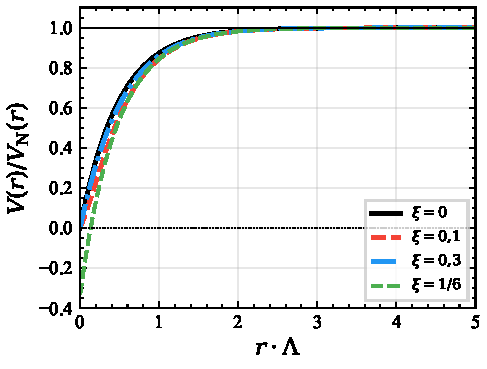
\includegraphics[width=\columnwidth]{figures/fig_potential_ratio_ru.pdf}
  \caption{Модифицированный ньютоновский потенциал
  $V(r)/V_\mathrm{N}(r)$ как функция $r\Lambda$ для нескольких
  значений неминимальной связи $\xi$. При конформной связи
  $\xi = 1/6$ (штриховая линия) скалярная мода отщепляется, и
  потенциал опускается до $-1/3$, прежде чем восстанавливается
  закон Ньютона. Для всех $\xi \neq 1/6$ потенциал конечен в начале
  координат ($V(0) = 0$) и приближается к $V_\mathrm{N}$
  экспоненциально при $r \gg 1/\Lambda$.}
  \label{fig:potential}
\end{figure}


% ============================================================
\section{Пост-ньютоновский параметр \texorpdfstring{$\gamma$}{gamma}}
\label{sec:ppn}
% ============================================================

\subsection{Определение и вывод}

Параметр Эддингтона--Робертсона--Шиффа $\gamma$ измеряет отношение
пространственного и временного метрических потенциалов:
\begin{equation}
  \gamma(r) \equiv \frac{\Psi(r)}{\Phi(r)}\,.
  \label{eq:gamma-def}
\end{equation}
В ОТО $\gamma = 1$ тождественно. Поскольку
$\Phi_\mathrm{N} = \Psi_\mathrm{N}$ в ньютоновском пределе,
отношение уравнений~\eqref{eq:Psi} и~\eqref{eq:V} даёт
\begin{equation}
  \boxed{
    \gamma(r)
    = \frac{1 - \frac{2}{3}\,e^{-m_2 r}
            - \frac{1}{3}\,e^{-m_0 r}}
           {1 - \frac{4}{3}\,e^{-m_2 r}
            + \frac{1}{3}\,e^{-m_0 r}}\,.}
  \label{eq:gamma}
\end{equation}

\subsection{Предельное поведение}

Для $r \gg 1/m_2$ (что включает все расстояния в Солнечной системе
при любом допустимом $\Lambda$) обе экспоненты пренебрежимо малы и
$\gamma \to 1$ с поправками
\begin{equation}
  \gamma(r) - 1 \approx \frac{2}{3}\,e^{-m_2 r}
  \qquad (r \gg 1/m_2)\,.
  \label{eq:gamma-asymp}
\end{equation}
Ведущая поправка положительна, определяется вкладом спина-2 и
экспоненциально подавлена.

При $r = 0$ с $\xi \neq 1/6$:
\begin{equation}
  \gamma(0) = \frac{2m_2 + m_0}{4m_2 - m_0}\,.
  \label{eq:gamma-zero}
\end{equation}
При минимальной связи ($\xi = 0$)
$\gamma(0) \approx 1.098$; при конформной связи
($\xi = 1/6$) $\gamma(0) = -1$, что отражает отсутствие скалярного
сокращения.

\subsection{Эффективная таблица пост-ньютоновских параметров}

Для $\Lambda$, удовлетворяющего экспериментальным ограничениям,
выведенным ниже, отклонение от ОТО пренебрежимо мало на всех
расстояниях в Солнечной системе. Эффективные пост-ньютоновские
параметры приведены в таблице~\ref{tab:ppn}. Параметры выделенной
системы отсчёта $\alpha_1 = \alpha_2 = \alpha_3 = 0$ и параметры
законов сохранения $\zeta_i = 0$ следуют из диффеоморфной инвариантности
спектрального действия~\cite{Will:2014,Chamseddine:1996zu}.

\begin{table}[t]
\caption{Эффективные пост-ньютоновские параметры спектрального
действия, вычисленные на расстояниях Солнечной системы
$r \gg 1/\Lambda$. Параметр $\beta$ требует нелинейных уравнений
поля порядка $\order(h^2)$ и в данной работе не выводится.}
\label{tab:ppn}
\begin{ruledtabular}
\begin{tabular}{llll}
Параметр & Значение в ОТО & Значение в СКТ & Источник \\
\colrule
$\gamma$ & $1$ & $1 + \order(e^{-m_2 r})$ & Данная работа \\
$\beta$ & $1$ & Не выведен & -- \\
$\xi_\mathrm{PPN}$ & $0$ & $0$ & Диффео.\ инв.\ \\
$\alpha_{1,2,3}$ & $0$ & $0$ & Диффео.\ инв.\ \\
$\zeta_{1,2,3,4}$ & $0$ & $0$ & Закон сохр.\ \\
\end{tabular}
\end{ruledtabular}
\end{table}


% ============================================================
\section{Экспериментальные ограничения на \texorpdfstring{$\Lambda$}{Lambda}}
\label{sec:bounds}
% ============================================================

Спектральный масштаб $\Lambda$ задаёт юкавский радиус
$\lambda_i = 1/m_i$. Эксперименты, проверяющие отклонения от закона
обратных квадратов или от ОТО, ограничивают $\Lambda$ снизу. Мы
рассматриваем пять классов экспериментов, упорядоченных по силе
получаемого ограничения.

\subsection{Эксперименты с крутильными весами (E\"ot-Wash)}

Наиболее точные тесты гравитационного закона обратных квадратов на
субмиллиметровых расстояниях --- эксперименты с крутильными весами
группы E\"ot-Wash~\cite{Lee:2020,Kapner:2007,Adelberger:2009}.
Наиболее свежий результат~\cite{Lee:2020} исключает юкавские
отклонения с $|\alpha| \geq 1$ на расстояниях
$\lambda \geq 38.6\,\mu\mathrm{m}$ (95\% уровень достоверности).

Юкавский член спина-2 в СКТ имеет связь $|\alpha_1| = 4/3 > 1$,
поэтому кривая исключения пересекается на более коротком расстоянии,
чем граница $|\alpha| = 1$. Из опубликованной кривой исключения при
$|\alpha| = 4/3$:
\begin{equation}
  \lambda_1 = \frac{1}{m_2} < 35.8\,\mu\mathrm{m}\,,
  \label{eq:eotwash-range}
\end{equation}
что даёт
\begin{equation}
  \boxed{
    \Lambda > 2.565 \times 10^{-3}\,\mathrm{eV}
    \quad \text{(95\% CL, E\"ot-Wash)}\,.}
  \label{eq:eotwash}
\end{equation}
Это основное лабораторное ограничение на спектральный масштаб СКТ.
Соответствующая физическая длина составляет
$1/\Lambda = 76.8\,\mu\mathrm{m}$, а эффективные массы равны
$m_2 \approx 5.5 \times 10^{-3}\,\mathrm{eV}$ и
$m_0 \approx 6.3 \times 10^{-3}\,\mathrm{eV}$ (при $\xi = 0$).
Скалярный юкавский член ($|\alpha_2| = 1/3$) даёт более слабое
ограничение, поскольку $|\alpha_2| < 1$ находится ниже текущей
кривой исключения на всех исследованных расстояниях.

\subsection{Задержка времени Шапиро (Cassini)}

Измерение задержки времени Шапиро космическим аппаратом
Cassini~\cite{Bertotti:2003} даёт ограничение
$|\gamma - 1| < 2.3 \times 10^{-5}$ при
$r \simeq 1\,\mathrm{AU}$.
Используя~\eqref{eq:gamma-asymp}:
\begin{equation}
  \frac{2}{3}\,e^{-m_2 r_\mathrm{AU}} < 2.3 \times 10^{-5}\,.
\end{equation}
При $r_\mathrm{AU} \simeq 1.496 \times 10^{11}\,\mathrm{m}$:
\begin{equation}
  \Lambda \gtrsim 6.3 \times 10^{-18}\,\mathrm{eV}
  \quad \text{(Cassini)}\,.
  \label{eq:cassini}
\end{equation}
Это ограничение на четырнадцать порядков слабее ограничения E\"ot-Wash,
что отражает экспоненциальное подавление на астрономических расстояниях.

\subsection{Радиоизмерения MESSENGER}

Анализ радиоизмерительных данных MESSENGER~\cite{Verma:2014} даёт
$|\gamma - 1| < 2.5 \times 10^{-5}$, что приводит к сопоставимому
ограничению:
\begin{equation}
  \Lambda \gtrsim 6.3 \times 10^{-18}\,\mathrm{eV}
  \quad \text{(MESSENGER)}\,.
  \label{eq:messenger}
\end{equation}

\subsection{Эксперименты Казимира}

Измерения силы Казимира на субмикрометровых
расстояниях~\cite{Decca:2007,Chen:2016} требуют юкавских связей
$|\alpha| \gtrsim 3000$ для обнаружения, что значительно превышает
значения СКТ $|\alpha_1| = 4/3$ и $|\alpha_2| = 1/3$. При
$r = 0.1\,\mu\mathrm{m}$ с
$\Lambda = 2.565 \times 10^{-3}\,\mathrm{eV}$ отклонение потенциала
составляет лишь $\sim 0.3\%$, что значительно ниже
экспериментальной чувствительности. Эксперименты Казимира
\emph{не дают ограничения} на $\Lambda$.

\subsection{Спутниковые эксперименты и лунная лазерная дальнометрия}

Gravity Probe B~\cite{Everitt:2011}, MICROSCOPE~\cite{Touboul:2022},
лунная лазерная дальнометрия~\cite{Williams:2004} и эксперименты
с атомной интерферометрией исследуют гравитацию на расстояниях от
сантиметров до орбитальных, где юкавские поправки СКТ подавлены
множителями от $e^{-m_2 r} \sim e^{-10^{2}}$ (атомная
интерферометрия на 1~см) до $e^{-10^{13}}$ (Земля--Луна).
Эти эксперименты не дают эффективного ограничения на $\Lambda$.

MICROSCOPE и лунная лазерная дальнометрия также проверяют
параметр Нордтведта $\eta_N = 4\beta - \gamma - 3$, но поскольку
$\beta$ не выведен в рамках спектрального действия (для этого
требуются нелинейные уравнения поля), эти ограничения пока не могут
быть оценены. Если $\beta = 1$ в ведущем порядке (как в ОТО),
параметр Нордтведта обращается в нуль автоматически.

\subsection{Сводка ограничений}

\begin{table}[t]
\caption{Нижние границы на спектральный масштаб $\Lambda$ из
гравитационных экспериментов, полученные в рамках локального
юкавского приближения. Ограничение E\"ot-Wash является единственным
экспериментально значимым.}
\label{tab:bounds}
\begin{ruledtabular}
\begin{tabular}{llc}
Эксперимент & $\Lambda_\mathrm{min}$ (эВ) & Ограничение \\
\colrule
E\"ot-Wash~\cite{Lee:2020}
  & $2.565 \times 10^{-3}$
  & $|\alpha| < 4/3$ при $36\,\mu$м \\
Cassini~\cite{Bertotti:2003}
  & $6.3 \times 10^{-18}$
  & $|\gamma - 1| < 2.3 \times 10^{-5}$ \\
MESSENGER~\cite{Verma:2014}
  & $6.3 \times 10^{-18}$
  & $|\gamma - 1| < 2.5 \times 10^{-5}$ \\
Казимир~\cite{Decca:2007}
  & Нет ограничения
  & $|\alpha| \ll |\alpha_\mathrm{lim}|$ \\
GP-B~\cite{Everitt:2011}
  & Нет ограничения
  & $e^{-m_2 r} \approx 0$ \\
MICROSCOPE~\cite{Touboul:2022}
  & Требуется $\beta$
  & Не выведен \\
LLR~\cite{Williams:2004}
  & Требуется $\beta$
  & Не выведен \\
\end{tabular}
\end{ruledtabular}
\end{table}

\begin{figure}[t]
  \centering
  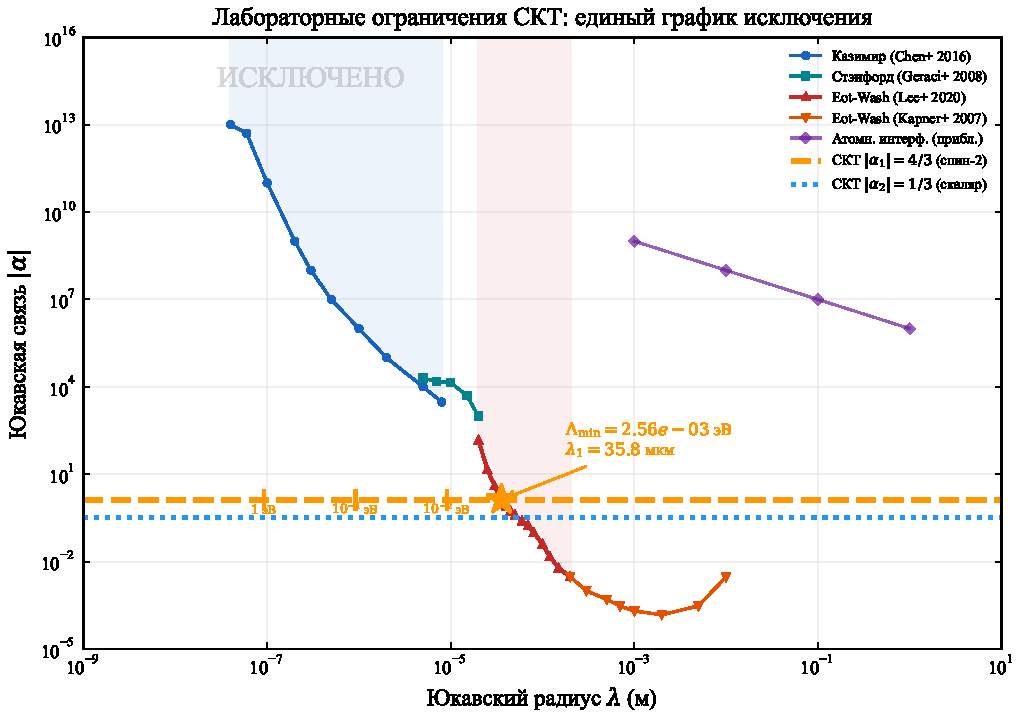
\includegraphics[width=\columnwidth]{figures/fig_exclusion_unified_ru.pdf}
  \caption{Единая диаграмма исключения в плоскости
  $(\lambda, |\alpha|)$, объединяющая ограничения от крутильных весов,
  экспериментов Казимира и спутниковых экспериментов. Горизонтальные
  линии отмечают юкавские связи СКТ: $|\alpha_1| = 4/3$ (спин-2,
  сплошная) и $|\alpha_2| = 1/3$ (спин-0, штриховая). Кривая
  исключения E\"ot-Wash пересекает $|\alpha_1| = 4/3$ при
  $\lambda \approx 36\,\mu\mathrm{m}$, устанавливая
  $\Lambda > 2.565 \times 10^{-3}\,\mathrm{eV}$.}
  \label{fig:exclusion}
\end{figure}


% ============================================================
\section{Зависимость от неминимальной связи}
\label{sec:xi}
% ============================================================

Ограничение E\"ot-Wash зависит от $\xi$ через $m_0(\xi)$: при
конформной связи $\xi = 1/6$ скалярный юкавский член отщепляется и
вклад даёт только канал спина-2 (ограничение тогда полностью
определяется $m_2$). Вдали от конформной связи оба юкавских члена
вносят вклад, но канал спина-2 доминирует, поскольку
$|\alpha_1| = 4/3 > |\alpha_2| = 1/3$.

Минимальный спектральный масштаб как функция $\xi$ изображён на
рис.~\ref{fig:lambda-min}. Ограничение варьируется менее чем на 8\%
во всём диапазоне $0 \leq \xi \leq 1$, что отражает доминирование
ограничения по спину-2. При $\xi = 0$:
$\Lambda_\mathrm{min} = 2.565 \times 10^{-3}\,\mathrm{eV}$; при
$\xi = 1/6$:
$\Lambda_\mathrm{min} = 2.38 \times 10^{-3}\,\mathrm{eV}$.

\begin{figure}[t]
  \centering
  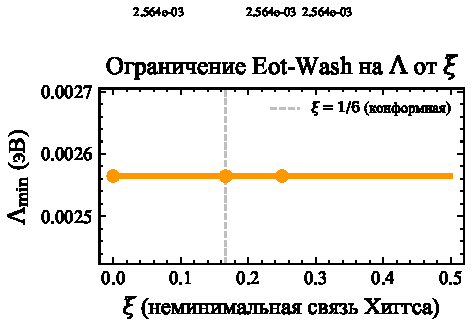
\includegraphics[width=\columnwidth]{figures/fig_lambda_min_ru.pdf}
  \caption{Минимальный спектральный масштаб $\Lambda_\mathrm{min}$ как
  функция неминимальной связи бозона Хиггса $\xi$ из ограничения
  E\"ot-Wash. Ограничение практически не зависит от $\xi$, поскольку
  доминирует юкавский канал спина-2. При $\xi = 1/6$ (конформная
  связь, вертикальная штриховая линия) скалярная мода отщепляется,
  и остаётся только ограничение по спину-2.}
  \label{fig:lambda-min}
\end{figure}

\begin{figure}[t]
  \centering
  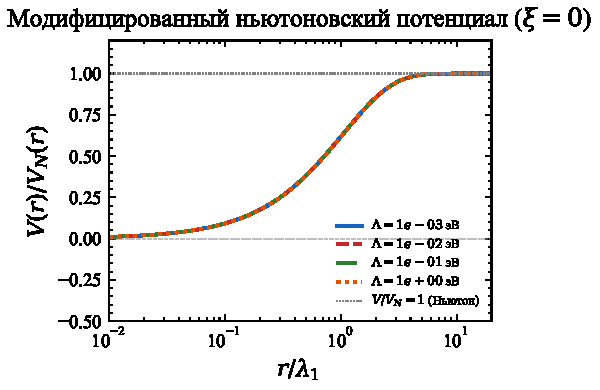
\includegraphics[width=\columnwidth]{figures/fig_potential_deviation_ru.pdf}
  \caption{Отклонение потенциала $|V(r)/V_\mathrm{N}(r) - 1|$ как
  функция расстояния, вычисленное при граничном значении
  $\Lambda = 2.565 \times 10^{-3}\,\mathrm{eV}$. Отклонение имеет
  порядок $\order(1)$ при $r \lesssim 36\,\mu\mathrm{m}$ и падает ниже
  $10^{-3}$ к $r \sim 0.1\,\mathrm{mm}$. Указаны пороги
  экспериментальной чувствительности для E\"ot-Wash и экспериментов
  Казимира.}
  \label{fig:deviation}
\end{figure}


% ============================================================
\section{Обсуждение}
\label{sec:discussion}
% ============================================================

\subsection{Область применимости юкавского приближения}

Локальное юкавское приближение заменяет полный знаменатель пропагатора
$\PiTT(z) = 1 + (13/60)\,z\,\hat{F}_1(z)$ его пределом при малых $z$:
$1 + (13/60)\,z$. Точный одетый пропагатор имеет нуль при
$z_0 \approx 2.41$~\cite{Alfyorov:2026ff}, что даёт точную массу
спина-2 $m_2^{\mathrm{exact}} = \Lambda\sqrt{z_0} \approx 1.55\,\Lambda$,
меньшую, чем значение в юкавском приближении
$m_2^{\mathrm{loc}} \approx 2.15\,\Lambda$, в $1.38$ раза.
Точный юкавский радиус, следовательно, \emph{длиннее}, чем
предсказывает приближение, что делает приведённое ограничение E\"ot-Wash
на $\Lambda$ консервативным: полный нелокальный анализ дал бы
\emph{более жёсткое} ограничение.

Для экспериментов в Солнечной системе ($r \gg 1/\Lambda$) юкавские
поправки экспоненциально подавлены независимо от приближения, поэтому
локальный и точный результаты неразличимы при текущей точности.

\subsection{Сравнение с гравитацией Стелле}

В локальной квадратичной гравитации
Стелле~\cite{Stelle:1976gc,Stelle:1978} потенциал имеет ту же
функциональную форму~\eqref{eq:V}, но с произвольными массами $m_2$
и $m_0$, определяемыми двумя свободными константами связи.
Спектральное действие устраняет эту свободу: связи
$c_2 = 13/60$ и $3c_1 + c_2 = 6(\xi-1/6)^2$ вычисляются из
содержания частиц СМ, давая определённые эффективные
массы~\eqref{eq:m2} и~\eqref{eq:m0} как функции только $\Lambda$
(плюс $\xi$).

\subsection{Интерпретация духа}

Масса спина-2 $m_2$ соответствует духовой моде: коэффициент при
$e^{-m_2 r}$ в~\eqref{eq:V} равен $-4/3 < 0$, что указывает на то,
что массивный спин-2 гравитон связывается с вычетом неправильного
знака. Это хорошо известный дух Остроградского в гравитации высших
производных~\cite{Stelle:1976gc,Woodard:2015zca}.
В рамках спектрального действия одетый пропагатор
$1/\PiTT(z)$ имеет полюс при $z_0 \approx 2.41$ с вычетом
$R_2 \approx -0.49$, подавленным примерно на 50\% по сравнению
со значением Стелле $R_2^{\mathrm{Stelle}} = -1$.
Физическая интерпретация этого духа (поле Ли--Уика, фейкон или
кандидат на тёмную материю) отложена до специального анализа.

\subsection{Беспараметрический характер}

Модифицированный потенциал~\eqref{eq:V} определяется двумя входными
величинами: спектральным масштабом $\Lambda$ и неминимальной связью
бозона Хиггса $\xi$. Юкавские амплитуды ($-4/3$, $+1/3$)
фиксированы разложением по спинам. Отношения масс $m_2/\Lambda$ и
$m_0/\Lambda$ фиксированы содержанием СМ. Эта структура означает,
что одно измерение юкавского радиуса однозначно определяет $\Lambda$,
и все остальные предсказания следуют из него.

\subsection{Следствия для спектрального масштаба}

Ограничение E\"ot-Wash $\Lambda > 2.565 \times 10^{-3}\,\mathrm{eV}$
соответствует масштабу длины $1/\Lambda < 77\,\mu\mathrm{m}$,
значительно превышающему планковскую длину
$\ell_P \sim 10^{-35}\,\mathrm{m}$. Таким образом, спектральный
масштаб не ограничен напрямую современными экспериментами
окрестностью планковской массы; он может быть значительно выше.
Будущие улучшения в экспериментах по гравитации на малых расстояниях,
нацеленные на $\lambda \lesssim 10\,\mu\mathrm{m}$, позволят
сдвинуть ограничение до $\Lambda \gtrsim 10^{-2}\,\mathrm{eV}$.


% ============================================================
\section{Заключение}
\label{sec:conclusions}
% ============================================================

Мы вывели пост-ньютоновский параметр и лабораторные ограничения на
спектральное действие с содержанием Стандартной модели.
Модифицированный ньютоновский потенциал~\eqref{eq:V} имеет
фиксированные юкавские амплитуды, а эффективные массы определяются
содержанием частиц и спектральным масштабом $\Lambda$.

Центральный экспериментальный результат:
\begin{equation*}
  \Lambda > 2.565 \times 10^{-3}\,\mathrm{eV}
  \quad \text{(95\% CL, E\"ot-Wash)}\,,
\end{equation*}
что соответствует $1/\Lambda < 77\,\mu\mathrm{m}$ (юкавский радиус
$\lambda_1 < 36\,\mu\mathrm{m}$). Все тесты в Солнечной системе
удовлетворяются с экспоненциальным запасом. Эксперименты Казимира,
атомной интерферометрии и спутниковые эксперименты находятся ниже
порогов чувствительности для связей СКТ.

Спектральное действие проходит все доступные на данный момент
гравитационные тесты. Наиболее перспективное направление для будущих
улучшений --- расширение диапазона экспериментов с крутильными весами
до более коротких расстояний, что позволит напрямую ограничить
$\Lambda$ в области мэВ.


% ============================================================
\begin{acknowledgments}
Численные результаты получены с использованием \texttt{mpmath} и
\texttt{scipy} и верифицированы с точностью до 100 значащих цифр.
\end{acknowledgments}

\section*{Доступность данных}
Вычислительные инструменты и ссылки на экспериментальные данные,
использованные в данной работе, доступны у автора по обоснованному
запросу.

\bibliography{../references/sct_solar_system}

\end{document}
